\documentclass{article}
\usepackage{fullpage}
\usepackage{amsmath,amssymb,amsfonts}
\usepackage{graphicx}
\usepackage{natbib}
\usepackage{xcolor}

\def\R{{\mathbb{R}}}
\def\pr{{\rm Pr}}
\def\E{{\mathbb E}}
\def\X{{\mathcal X}}
\def\Y{{\mathcal Y}}
\def\H{{\mathcal H}}
\def\G{{\mathcal G}}
\def\B{{\mathcal B}}
\def\bias{{\rm bias}}
\def\supp{{\rm supp}}
\def\yh{{\widehat{y}}}
\def\PL{{\rm PL}}

\newtheorem{thm}{Theorem}
\newtheorem{lemma}[thm]{Lemma}
\newtheorem{cor}[thm]{Corollary}
\newtheorem{claim}[thm]{Claim}
\newtheorem{defn}[thm]{Definition}
\newtheorem{assump}{Assumption}
\newtheorem{open}{Open problem}
\newenvironment{proof}{\noindent {\sc Proof:}}{$\Box$ \medskip}

\newcommand{\sanjoy}[1]{{\color{red} {\bf Sanjoy:} #1}}
\newcommand{\yoav}[1]{{\color{blue} {\bf Yoav:} #1}}

\DeclareMathOperator*{\argmax}{arg\,max}

\title{Active learning using the near-Neighborhoods algorithm}

\begin{document}

\maketitle
\section{Setup}

\begin{enumerate}
\item {\it Pool-based active learning.}

\begin{itemize}
\item We have a finite dataset $X$ of $n$ points, and we are able to query the labels of any of them.
\item We want a procedure that chooses the next point, or batch of points, to query. This process might be stopped at any time, and then the remaining labels will need to be inferred.
\item The goal is for the inferred labels to converge to their ``gold-standard'' values (to be defined) as quickly as possible, ideally much faster than would occur if the query points were chosen uniformly at random.
\end{itemize}

\item {\it Model of data.}

\begin{itemize}
\item The dataset $X$ consists of $n$ independent samples from a fixed but unknown distribution $\mu$ on a metric space $(\X, d)$. 
\item Label space $\Y = \{-1,+1\}$. Each $x \in \X$ is labeled according to conditional probability function $\eta(x) = \pr(Y=1|X=x)$, also unknown.
\item The Bayes-optimal classifier on $\X$ is $g^*(x) = \mbox{sign}(2 \eta(x) - 1)$. This is the gold-standard for inferred labels.
\end{itemize}


\end{enumerate}

s\section{Deterministic algorithm}

\begin{enumerate}
\item Define the highest level to be $l_{max} = \log_2 n$.
\item We have a collection of balls $\B$, organized into levels $\B_\ell$, where $\ell = 0, 1, 2, \ldots$. $\B_\ell$ contains all balls whose probability (wrt the uniform distribution over the examples) satisfies $\frac{1}{2^l} \leq p(B) < \frac{1}{2^{l-1}}$
\item We define $\eta(B) = \pr(Y=1|X \in B)$,
%We will use the shorthand
%$$ \B_{\leq \ell} = \bigcup_{\ell' \leq \ell} \B_{\ell'} $$
%to denote balls upto and including level $\ell$.

\item Let $\B(x) \subset \B$ denote the balls that may be consulted in determining the label of point $x$. These could, for instance, be all balls that contain $x$. Or they could be all balls centered at some $x \in X$

\item The algorithm can query an oracle for a (of labels) for a set of balls $Q_\ell \subset \B_\ell$. The oracle responds with a set of data points such that there are at least $k$ independent samples in each ball $B \in Q_\ell$.

\item
Using these samples we can label each ball in $Q_\ell$ as $y(B)=+1/0/-1$ such that, with probability of $Q_\ell$ such that with probability $1-\delta$ and for some $\epsilon>0$ the following holds for each $B \in Q_\ell$: 
\begin{itemize}    
\item $y(B) = +1 \implies \eta(B) \geq 1-\epsilon$
\item $y(B) = -1 \implies \eta(B) \leq \epsilon$
\item $y(B) = 0 \implies |\eta(B)-1/2| \leq \epsilon$
\end{itemize}

\item Once we have queried all balls in $\B_{\ell}(x)$, we determine the set of possible labels of $x$ at level $\ell$, denoted $\PL_\ell(x) \subset \{-1,+1\}$. It is defined as follows:
\begin{itemize}
\item $\PL_\ell(x)$ contains $+1$ iff there exists $B \in \B_{\ell}(x)$ with $y(B) = +1$ and there is  no $B' \in \B_{ \ell}(x)$ has both $B' \subset B$ and $y(B') = -1$.
\item A similar condition determines whether $\PL_\ell(x)$ contains $-1$.
\item
Given this set of possible labels of $x$, we assign a label
$$ y_\ell(x)
=
\left\{
\begin{array}{cl}
+1 & \mbox{if $+1 \in \PL_\ell(x)$  and $-1 \notin \PL_\ell(x)$}\\
-1 & \mbox{if $-1 \in \PL_\ell(x)$  and $+1 \notin \PL_\ell(x)$}\\
0 & \mbox{if $\PL_\ell(x) = \{0\}$} \\
! & \mbox{if $+1 \in \PL_\ell(x)$  and $-1 \in \PL_\ell(x)$}
\end{array}
\right.
$$
\item Define $U_\ell = \{x \in X: y_{\ell-1}(x) = !\}$
\item Define the set of query balls 
$$Q_l= \left\{B \in \B_l  |   B \cap U_{l-1} \neq \emptyset \right\}$$
And define the focus set to be the union of the query balls:
$$F_l = \bigcup_{B \in Q_l} B$$
\end{itemize}

\item Implementing the oracle. Let $P_\ell = \Pr[F_\ell]$
Our hypothesis is that, if the set of balls has $d$, if we we select $M_\ell = C (\log d \log \delta^{-1})(n k 2^\ell) P_\ell$ independent points in $F_\ell$ then with probability at least $1-\delta$ each ball contains at least $k$ samples.

\item Deterministic algorithm\\
Set $F_1 = X$  \\
For $l=1,\ldots, l_{max}$
\begin{itemize}
\item {\em Focused Query:} Query $M_\ell$ from $F_\ell$
\item {\em Uniform query:} Query $M_\ell$ from $X$
\item {\em Back-filling:} Consider a "hindsight known unknown" to be a set 
$U_m \neq \emptyset$ for $m<\ell$ that was not identified in iteration $\ell-1$. Then focused sampling is added for levels $m+1$ till $\ell$. (needs clearer explanation)
\end{itemize}
\end{enumerate}

\section{Sketch of analysis}

Consider the number of focused queries made at level $\ell$: $M_\ell = C (\log d \log \delta^{-1})(n k 2^\ell) P_\ell$.
Denote $N_\ell = 2C (\log d \log \delta^{-1})(n k 2^\ell)$. Then $M_{\ell} = N_\ell P_\ell$. is the number of samples needed to guarantee that the balls in $Q_\ell$ all contain at least $k$ samples. 
If we replace $P_\ell$ with $1$ we get $N_l$: the number of uniform queries needed to get reliable labels for all 
of the balls in $\B_\ell$.

Fix a point $x\in X$, define the history $H(x)$ to be as binary sequence of length $l_{max}$ where each element is either 
$C$ for {\em consistent} or $I$ for {\em Inconsistent}.  We use $H_i(x)$ to indicate the $i$'th element in $H(x)$.
$H_i(x)=I$ if and only if $x \in F_\ell$.

We now characterize the convergence of the predictions on $x$.  We say that $c(x)$ is the {\em convergence point for $x$} if $j=c(x)$ is the smallest integer such that for all $i\geq j$, $H_i(x)=C$. we say that $d(x)$ is the {\em final disagreement point} if $j=d(x)$ is the smallest integer such that for all $j \geq i > c(x)$, $H_j(x)=I$

Our analysis is based on the following intuition. For levels $1,\ldots,d(\ell)-1$ we need to use uniform sampling while for levels $d(\ell),\ldots c(\ell)-1$ we use focused sampling.

As a result the number of samples needed is 
$$ 2\left( \sum_{\ell=1}^{d(x)-1} N_{\ell} + \sum_{\ell=d(x)}^{c(x)-1} N_\ell P_\ell \right) $$ while the number of queries needed  using standard uniform queries is  
$$ \sum_{\ell=1}^{c(x)-1} N_{\ell} $$
Easy examples are ones where the $d(x)$ and $c(x)$ are small and $P_\ell$ is small for $d(x)\geq \ell \geq c(x)$. Note that the sequence $P_1,P_2$ is global and does not depend on $x$. The dependence on $x$ comes in through $d(x)$ and $c(x)$
\pagebreak
\section{1D example}
I believe that for each point $x$ there are two critical levels. In the following I say that balls are "in agreement" if there is a sign $s \in \pm 1$ such that each ball is labeled either $s$ or $?$
\begin{itemize}
    \item The convergence level: all balls at this or higher level are in agreement with the polarity same $s$.
    \item The last unknown-unknown level: the highest level in which there is agreement and the label is wrong.
\end{itemize}
Basically, we rely on uniform sampling until we pass the last unknown-unknown level. We rely on focused sampling from that level until convergence.

In the figure above I sketch a simple case where there are two thresholds and $\eta$ is either $1/2-\gamma$ or $1/2+\gamma$. In this case the convergence radius is $d/2$ and the last UU is radii above $2W$

\begin{figure}[t]
\begin{center}
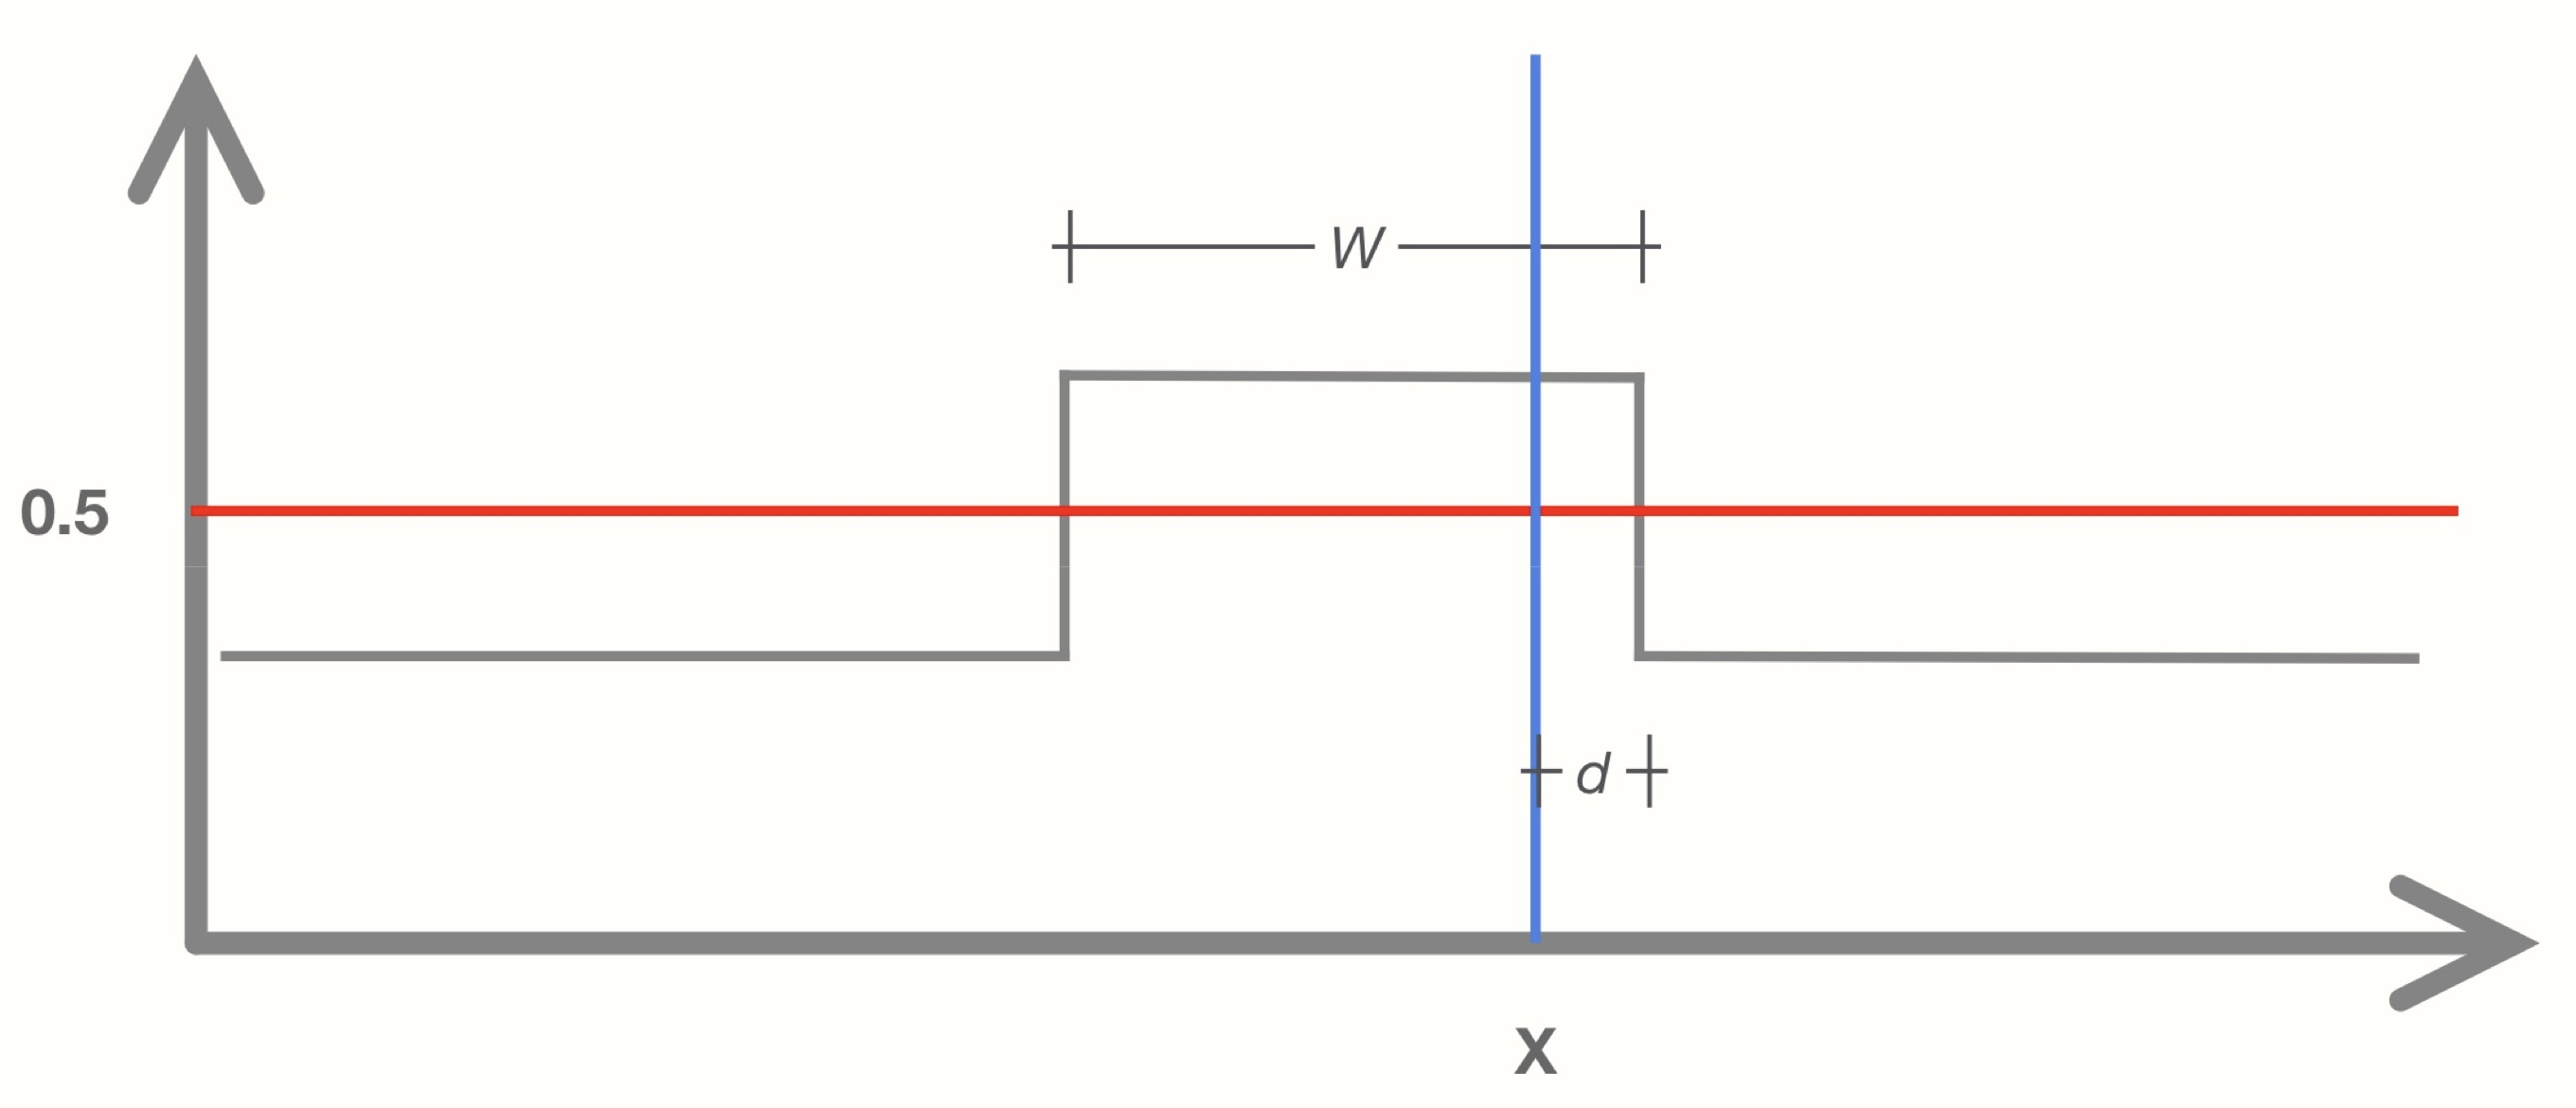
\includegraphics[width=4in]{1Dbump.jpg}
\end{center}
\label{fig:cases}
\end{figure}

\section{Active learning algorithm}

\subsection{Some details}

\begin{enumerate}

\item {\it Sampling regions.}
The sampling is organized around a collection $\B$ of measurable subsets of $\X$. These are the atomic sets on which we assess label bias and we call them ``balls''.

\begin{enumerate}

\item[(a)] {\it Points within a ball.} For any ball $B \in \B$, let $X_B$ denote the points in $X$ that can be used to assess the bias of $B$. This is simply $X_B = X \cap B$ unless $\B$ is constructed in a way that depends on $X$ and causes certain points to be excluded.\footnote{The construction of $\B$ may or may not depend on the unlabeled points $X$, and this distinction determines which points can be considered random draws from a particular $B \in \B$. For instance, consider these two alternatives for defining $\B$:
\begin{itemize}
\item $\B$ consists of a pre-defined set of balls.
\item $\B$ consists of balls defined by pairs of points in $X$, with each $x,x' \in X$ yielding the ball $B(x,\|x-x'\|)$.
\end{itemize}
In the first case, all points $X \cap B$ are random draws from $B$. In the second case, this is also true except for the two points $x,x'$ that define the ball.}

\item[(b)] {\it Grouping balls by size.} We will group balls by the number of points that they contain: we put $B$ at {\it level} $\ell$ if
$$ \frac{n}{2^{\ell + 1}} \leq |X_B| < \frac{n}{2^\ell} .$$
Here $\ell$ ranges from $0$ (consisting of balls that contain at least half the data points) to roughly $\lg n$ (containing a single point). 

Let $\B_\ell$ consist of all balls in $\B$ that are at level $\ell$. Thus $\B_0, \B_1, \ldots$ is a partition of $\B$, with $\B_0$ consisting of very large balls and subsequent $\B_1, \B_2, \ldots$ consisting of successively smaller balls.

\item[(c)] {\it Balls used to evaluate a given point.}

For any $x \in \X$, let $\B(x) \subset \B$ denote the collection of balls that will be used in determining $x$'s label. There are many ways in which this could be set, for instance,
\begin{itemize}
\item all balls containing $x$, or
\item all balls centered at $x$.
\end{itemize}
As before, we can partition these balls by sampling-level, so that $\B_\ell(x) = \B(x) \cap \B_\ell$.

\end{enumerate}

\item {\it Bias-estimates for balls and for data points.} The active learning algorithm uses label-queries to assess the bias of balls $B \in \B$. In turn, these are used to estimate the labels of individual points.

\begin{enumerate}

\item[(a)] {\it Bias of a ball.} The bias of a ball $B \in \B$ is defined as
$$ \eta_X(B) = \mbox{average}\{\eta(x): x \in X_B \} .$$

\item[(b)] {\it Qualitative estimates of bias.} Each ball $B$ is assigned qualitative bias estimate,
$$ \yh(B) = 
\left\{
\begin{array}{cl}
+1 & \mbox{significant $+$ bias} \\
-1 & \mbox{significant $-$ bias} \\
0 & \mbox{no significant bias} \\
\bot & \mbox{not yet available}
\end{array}
\right.
$$
The option $\bot$ is used until sufficiently many points in $X_B$ have been labeled: the required number, $k$, is roughly $1/\gamma^2$ (recall that $\gamma$ is the smallest bias that needs to be detected). Once $k$ labels are available, $\yh(B)$ is set to a value in $\{-1,0,+1\}$ and remains fixed thereafter.

\item[(c)] {\it Bias guarantees.} Our bias estimates will satisfy a guarantee of the following form: with probability $1-\delta$, for all $B \in \B$, once $\yh(B)$ is set to a value in $\{-1,0,+1\}$, 
\begin{itemize}
\item $\yh(B) = +1 \implies \eta_X(B) > b_1$
\item $\yh(B) = -1 \implies \eta_X(B) < -b_1$
\item $\yh(B) = 0 \implies |\eta_X(B)| < b_2$
\end{itemize}
for some constants $0 < b_1 < b_2 < 1$.

\item[(d)] {\it Possible labels for a point.} Pick any $x$ and any level $\ell$. Once bias-estimates are available for all balls $B \in \B_\ell(x)$, the possible labels for $x$ at level $\ell$ are $\PL_\ell(x) \subset \{-1,+1\}$, defined as follows:
\begin{itemize}
\item $\PL_\ell(x)$ contains $+1$ if and only if there exists $B \in \B_\ell(x)$ with $y(B) = +1$ such that there is no $B' \in \B_\ell(x)$ with $B' \subset B$ and $y(B') = -1$.
\item $\PL_\ell(x)$ contains $-1$ is defined symmetrically.
\end{itemize}

\item[(e)] {\it The label of a point at level $\ell$.} The label of point $x$ at level $\ell$ is a value $\yh_\ell(x) \in \{-1,+1,0,!,\bot\}$. It is initially $\bot$, but once bias-estimates are available for all $B \in \B_\ell(x)$, it is set to a value in $\{-1,+1,0,!\}$ and remains fixed thereafter:
\begin{equation}
\yh_\ell(x) = 
\left\{
\begin{array}{cl}
+1 & \mbox{if $\PL_\ell(x) = \{+1\}$} \\
-1 &  \mbox{if $\PL_\ell(x) = \{-1\}$} \\
0 & \mbox{if $\PL_\ell(x) = \{\}$} \\
! & \mbox{if $\PL_\ell(x) = \{-1,+1\}$}
\end{array}
\right.
\label{eq:provisional-label}
\end{equation}
Points labeled $!$ are ``known unknowns'': they are near the decision boundary and need further investigation. Points labeled $0$ show no significant bias.

\end{enumerate}

\end{enumerate}

\subsection{The algorithm}

\begin{figure}[h!]
\framebox{
\begin{minipage}[t]{6.4in}
\begin{itemize}
\item Initialize uncertainty regions at all levels:
\begin{itemize}
\item $U_0 = X$
\item $U_\ell = \emptyset$ for $\ell \geq 1$
\end{itemize}

\vspace{.1in}
\item Repeat:
\begin{itemize}
\item If there is a level $\ell \geq 0$ such that $U_\ell \neq \emptyset$:
\begin{itemize}
\item Let $\ell'$ be the smallest such level
\item {\tt Focused-query}($\ell', U_{\ell'}$)
\end{itemize}
\item {\tt Background-query}
\item Update $\yh_{\ell}$ values, $\ell \geq 0$, as per equation (\ref{eq:provisional-label})
\item $U_0 = \{x \in X: \yh_0(x) = \bot\}$
\item For all levels $\ell \geq 1$: $U_\ell = \{x \in X: \yh_{\ell-1}(x) = \,!, \ \yh_\ell(x) = \bot\}$
\end{itemize}

\end{itemize}

\end{minipage}}
\caption{The active learning algorithm. In each iteration, (at most) one focused query and one background query are made.}
\label{alg:main}
\end{figure}


\begin{figure}[h!]
\framebox{
\begin{minipage}[t]{6.4in}

\vspace{.1in}
\emph{Initialization:}
\begin{itemize}
\item Set $Q = \emptyset$ (points queried so far)
\item For each $x \in X$: choose $T_x \sim \mbox{unif}[0,1]$
\end{itemize}

\vspace{.2in}
{\bf Focused-query}($\ell, U$)

\vspace{.1in}
\begin{itemize}
\item Query region:
$$ S =  \bigcup_{x \in U} \bigcup_{B \in \B_\ell(x)} \{z \in X_B: T_z \leq \tau_\ell\} $$
\item Query the next unlabeled point in $S \setminus Q$, ordered by $T_z$ values, and add to $Q$
\end{itemize}

\vspace{.2in}
{\bf Background-query}

\vspace{.1in}
\begin{itemize}
\item Query the next unlabeled point in $X \setminus Q$, ordered by $T_z$ values, and add to $Q$
\end{itemize}

\end{minipage}}
\caption{The sampling procedures. Each point $x \in X$ has an associated value $T_x$ chosen uniformly at random from $[0,1]$. This smaller this value, the earlier this point is likely to be queried. The focused querying procedure also uses threshold $\tau_\ell = 2^{\ell+2}k/n$.} 
\label{alg:sampling}
\end{figure}


\section{Analysis of algorithm}

\subsection{Accuracy of bias estimates}

We'll start with a uniform guarantee on the bias estimates for all balls $B \in \B$.

Recall that each point $x \in X$ gets a label $Y \in \{-1,+1\}$ according to the distribution
$$ \eta(x) = \E[Y | X=x].$$ 
For any $B \in \B$ with $X_B \neq \emptyset$, let $\eta_X(B)$ be the average $\eta$-value in $B$, that is,
$$ \eta_X(B) = \frac{1}{|X_B|} \sum_{x \in X_B} \eta(x) .$$
The specific property we need is encapsulated in the following definition.
\begin{defn}
For any $B \in \B$ and $0 < b_1 < b_2$, we say bias estimate $\yh(B) \in \{+1,-1,0\}$ is \emph{$(b_1,b_2)$-accurate} if the following holds:
\begin{itemize}
\item $\yh(B) = +1 \implies \eta_X(B) > b_1$
\item $\yh(B) = -1 \implies \eta_X(B) < -b_1$
\item $\yh(B) = 0 \implies |\eta_X(B)| < b_2$
\end{itemize}
\label{def:accurate-bias-estimate}
\end{defn}

In what follows, take $0 < \delta < 1$ to be a predefined constant, and define
\begin{equation}
c_1 = \sqrt{3 \ln \frac{4|\B|}{\delta}} .
\label{eq:c1}
\end{equation}

For any level $\ell$, define threshold $\tau_\ell$ as follows:
\begin{equation}
\tau_\ell = \min \left( \frac{2^{\ell+2}k}{n}, \ 1 \right)
\label{eq:threshold-ell}
\end{equation}
For any $B \in \B_\ell$, define its \emph{query-set} to be $\Gamma(B) = \{z \in X_B: T_z \leq \tau_\ell\}$. We base our bias-estimate for $B$ on the labels of points in $\Gamma(B)$.

Our main deviation bound is the following, a consequence of Lemma~\ref{lemma:large-deviation-discrete} in the appendix.
\begin{thm}
Suppose $k \geq 2c_1^2$. With probability at least $1-\delta$, the following is true for all $B \in \B$ with $|X_B| \geq k$:
\begin{enumerate}
\item[(a)] The query set $\Gamma(B)$ has size at least $k$.
\item[(b)] The average label on $\Gamma(B)$, call it $\widehat{\eta}(B)$, satisfies
$$ \left| \widehat{\eta}(B) - \eta_X(B) \right| \leq \frac{4c_1}{\sqrt{k}}.$$
\end{enumerate}
\label{thm:large-deviation-bounds}
\end{thm}
\begin{proof}
These follow immediately by applying Lemma~\ref{lemma:large-deviation-discrete} to each $B \in \B$ and taking a union bound. 
\end{proof}

The following corollary of Theorem~\ref{thm:large-deviation-bounds} is immediate.
\begin{cor}
Suppose that $k \geq (8c_1/(b_2-b_1))^2$ where $c_1$ is given in (\ref{eq:c1}). 
For each $B \in \B$, let $\widehat{\eta}(B)$ be the average label on the query-set $\Gamma(B)$, and define the bias-estimate $\yh(B)$ as follows:
$$ \yh(B)
= 
\left\{
\begin{array}{ll}
\mbox{sign}(\widehat{\eta}(B)) & \mbox{if $|\widehat{\eta}(B)| \geq (b_1 + b_2)/2$} \\
0 & \mbox{otherwise}
\end{array}
\right.
$$
With probability $\geq 1-\delta$, all bias estimates $\yh(B)$, for $B \in \B$, are $(b_1,b_2)$-accurate.
\label{cor:accurate-bias-estimates}
\end{cor}
In what follows, we will assume that this $(1-\delta)$-probability event holds.



\pagebreak

\begin{figure}
\begin{center}
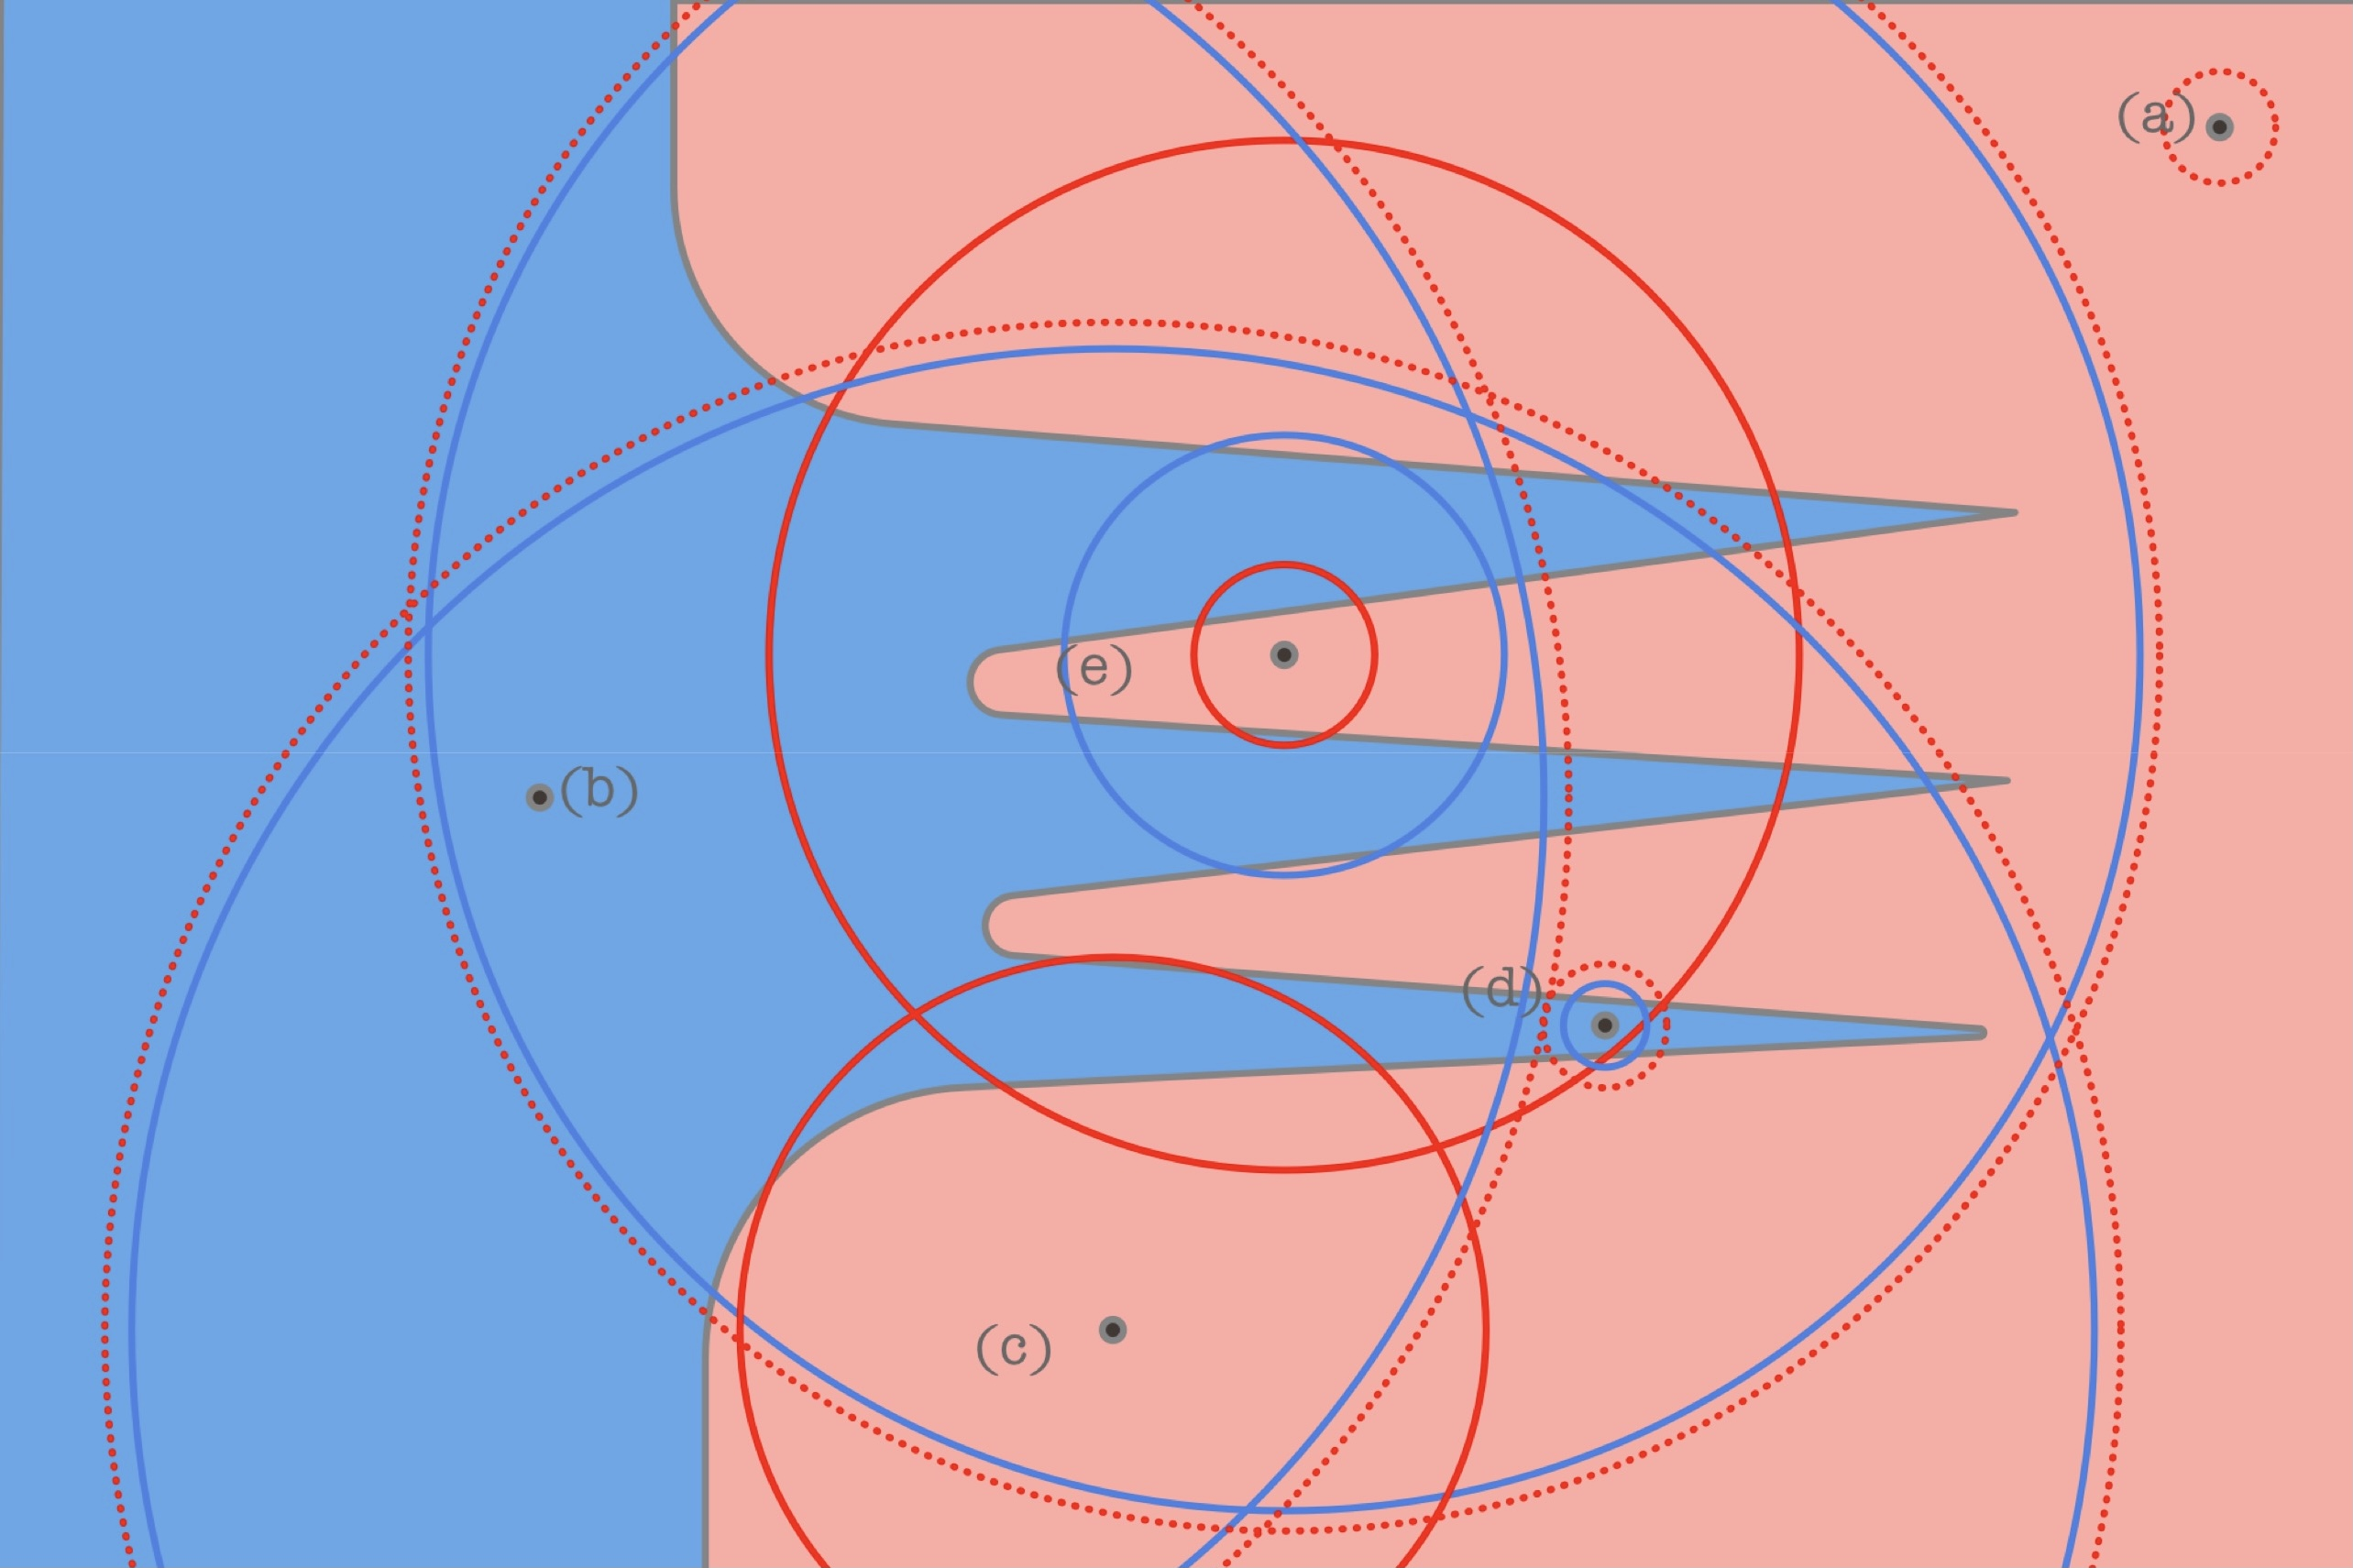
\includegraphics[width=6in]{IMG_0840.jpg}
\end{center}

\caption{This figure provides some examples for the concept of mind changes. Here we consider true probabilities, rather than estimates. The bounding rectangle defines the input space $X$. The blue region indicate $x$'s where the probability of +1 is larger than that of $-1$, the red region indicates the revers polarity. More specifically, we assume that in the blue region the probability of +1 is 0.6, while in the red region the probability of +1 is 0.4.
The black dots correspond to points on which we want to make a prediction. We consider all circles centered at each point. The {\em bias} of  circle is the probability of +1 conditioned on the point being in the circle. As labels are accumulated, the bias of smaller and smaller circles can be determined. For any point there is a large enough circle that contains the whole input space. We assume that the overall bias is negative, hence for a sufficiently large circle the bias is negative. This is indicated by the dotted circle which is always the largest circle. The solid line circles are the largest circles with the polarity indicated by the color of the line. The smallest circle corresponds to the last mind change which we also call the convergence circle.
A point is considered "easy" if its convergence circle is large, because that means that a small number of queries is required to find the correct label.
Following that definition we get that the order of points from the easiest to the hardest is {\bf a,b,c,e,d}. Comparing e and d we see that d has a smaller convergence circle, and one mind change, which (e) has a larger convergence circle, but has 4 mind changes.
}

\label{fig:mind-changes}
\end{figure}

\iffalse
\begin{figure}
\begin{center}
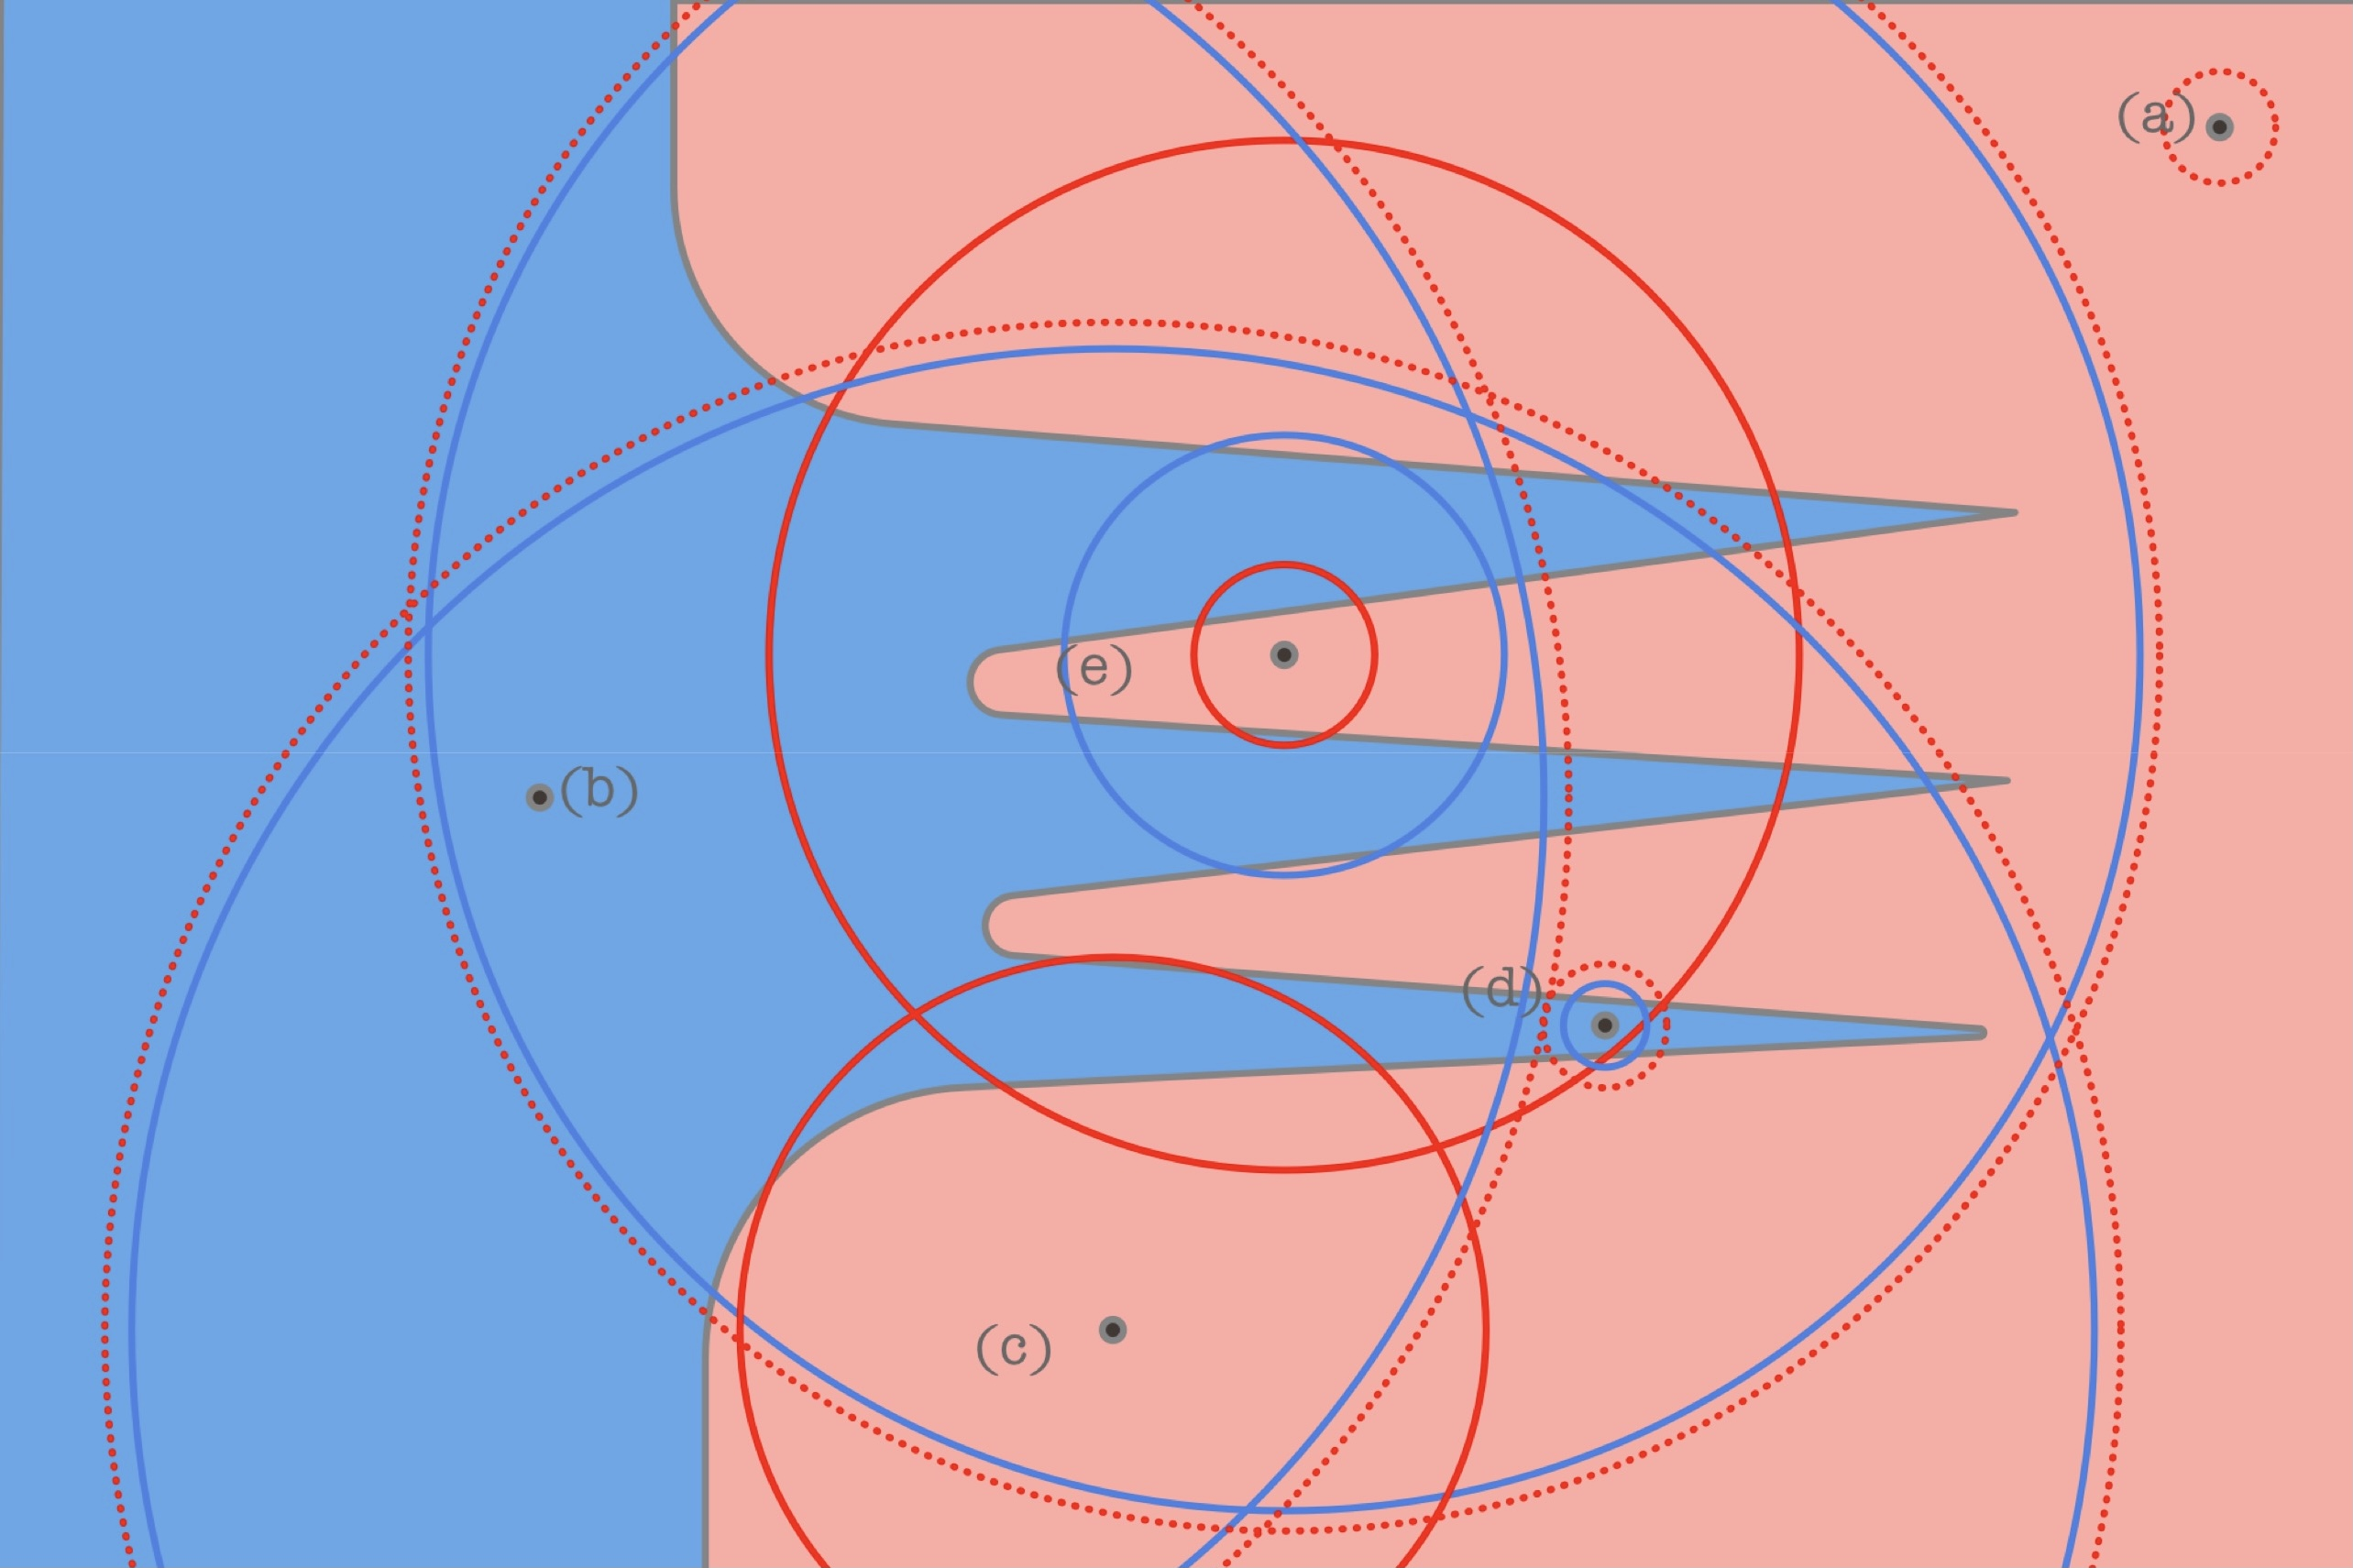
\includegraphics[width=6in]{IMG_0840.jpg}

%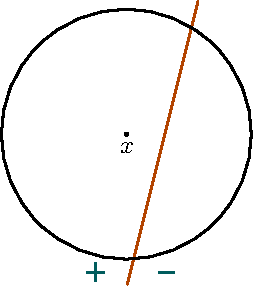
\includegraphics[width=1.5in]{boundary3.pdf}
%\hskip1in
%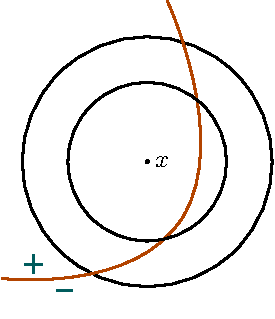
\includegraphics[width=1.75in]{boundary4.pdf}
\end{center}
\caption{\emph{Left:} In this picture, it could be the case that every ball $B \in \B(x)$ has $\eta(B) \geq 1/2$, in which case $L_s(x) = 0$. But these balls may not have significant positive bias until a higher level $L_f(x)$ (which includes the shown ball). \emph{Right:} This is a situation in which, for small $\ell$, balls $B \in \B_\ell(x)$ might have $\eta(B) < 1/2 - \gamma$. But for $\ell \geq L_s(x)$, we get balls (such as the outer ball) with a positive bias, and for $\ell \geq L_f(x)$ (such as the inner ball), a significant positive bias.}
\label{fig:critical-interval}
\end{figure}
\fi


\section{Technicalities}

\subsection{Large deviation bounds}

\begin{lemma}
Fix a confidence parameter $0 < \delta < 1$ and a positive integer $k \geq 6 \ln (4/\delta)$. 

Let $x_1, \ldots, x_m$ be any collection of points. Suppose that the labels $Y_i \in \{-1,1\}$ of these points are independent, with $\E Y_i = \eta(x_i)$. Define
$$ \eta_o = \frac{1}{m} \left( \eta(x_1) + \cdots + \eta(x_m) \right) .$$
Now consider the following estimator $Z$ of this quantity:
\begin{itemize}
\item Each $x_i$ is chosen with probability $q > 0$, independently. Let $N$ be the number of selected points.
\item If $N > 0$, the labels $Y_i$ of the selected points are obtained, and $Z$ is their average.
\end{itemize}
If $qm \geq k + \sqrt{6k \ln (4/\delta)}$, with probability at least $1-\delta$, 
\begin{enumerate}
\item[(a)] $N \geq k$, and 
\item[(b)] $| Z - \eta_o| \leq \sqrt{(48/k) \ln (4/\delta)}$.
\end{enumerate}
\label{lemma:large-deviation-discrete}
\end{lemma}
\begin{proof}
Let's start with (a). Define $c_1 = \sqrt{3 \ln (4/\delta)}$. We'll take $qm = k + \sqrt{6k \ln (4/\delta)} = k + c_1 \sqrt{2k}$ since this is the worst case. By assumption, $k \geq 2c_1^2$ and thus $qm \leq 2k$.

Now, $N$ has a binomial($m,q$) distribution. By a multiplicative Chernoff bound, for $0 < \epsilon < 1$, we have
\begin{align*}
\pr(N \geq qm(1+\epsilon)) &\leq e^{-qm\epsilon^2/3} \\
\pr(N \leq qm(1-\epsilon)) &\leq e^{-qm\epsilon^2/2}
\end{align*}
Take $\epsilon = c_1/\sqrt{qm}$; by the lower bound on $k$, we have $\epsilon \leq 1/2$. Recalling the choice of $c_1$, we see that with probability at least $1-\delta/2$, we get 
$$(1-\epsilon) qm < N < (1+\epsilon) qm .$$
The lower bound implies $N > qm(1-\epsilon) = qm - c_1\sqrt{qm} = k + c_1 \sqrt{2k} - c_1 \sqrt{qm} \geq k$.

For (b), define $C_1, \ldots, C_m \in \{0,1\}$ as random variables indicating whether the corresponding points were selected; that is, $C_i = {\bf 1}(\mbox{$x_i$ was selected})$. The sum of the obtained labels is then $S = C_1 Y_1 + \cdots + C_m Y_m$. Notice that these $C_iY_i \in \{-1,0,1\}$ are independent with $\E[C_iY_i] = q \eta(x_i)$ and $\E[(C_iY_i)^2] = \E[C_i] = q$. Thus their sum $S$ has expectation
$$ \E [S] = \sum_{i=1}^m \E[C_i Y_i] = \sum_{i=1}^m q \eta(x_i) = qm \eta_o $$
and variance
$$ \mbox{var}(S) = \sum_{i=1}^m \mbox{var}(C_iY_i) \leq qm .$$
We can bound the concentration of $S$ around its expected value using Bernstein's inequality, by which
$$ \pr(|S - \E[S]| \geq t) \leq 2 \exp \left( - \frac{t^2}{2(\mbox{var}(S) + 2t/3)} \right) .$$
Using $t = \epsilon qm$, we then have that $|S - qm \eta_o| \leq \epsilon qm$ with probability at least $1-\delta/2$.

Combining with the high-probability bound on $N$ above, we get
$$ \frac{qm \eta_o - \epsilon qm}{qm(1+\epsilon)} < \frac{S}{N} < \frac{qm \eta_o + \epsilon qm}{qm(1-\epsilon)},$$
whereupon (recalling $Z = S/N$)
$$ 
\eta_o \left( \frac{1}{1+\epsilon} -1 \right) - \frac{\epsilon}{1+\epsilon} < Z - \eta_o < \eta_o \left( \frac{1}{1-\epsilon} - 1 \right) + \frac{\epsilon}{1-\epsilon} .$$
Since $|\eta_o| \leq 1$,
$$ |Z - \eta_o | \leq \max \left( \frac{2\epsilon}{1+\epsilon}, \frac{2\epsilon}{1-\epsilon} \right)
\leq 
4 \epsilon,$$
as claimed.  
\end{proof}



\end{document}
